\documentclass[aspectratio=169]{beamer}
\usepackage[utf8]{inputenc}
\usepackage{utopia} %font utopia imported
\usetheme{Madrid}
\usecolortheme{default}

\usepackage{pgfplots}
\usepackage{tikz}
\usepackage[european resistor, european voltage, european current]{circuitikz}
\usetikzlibrary{arrows,shapes,positioning}
\usetikzlibrary{decorations.markings,decorations.pathmorphing,
decorations.pathreplacing}
\usetikzlibrary{calc,patterns,shapes.geometric}

%Information to be included in the title page:
\title{Cours d'introduction à la chimie quantique}

\subtitle{Chapitre 4 : Atome hydrogénoide\\Partie 1 :Fonction radiale}
\author{François Dion}
%\institute{Overleaf}
\date{2020}




%\logo{\includegraphics[height=1.5cm]{lion-logo.jpg}}

%End of title page configuration block
%------------------------------------------------------------



%------------------------------------------------------------
%The next block of commands puts the table of contents at the 
%beginning of each section and highlights the current section:

%\AtBeginSection[]
%{
  %\begin{frame}
    %\frametitle{Table of Contents}
    %\tableofcontents[currentsection]
  %\end{frame}
%}
%------------------------------------------------------------


\begin{document}

%The next statement creates the title page.
\frame{\titlepage}


%---------------------------------------------------------
%This block of code is for the table of contents after
%the title page
%\begin{frame}
%\frametitle{Table of Contents}
%\tableofcontents
%\end{frame}
%---------------------------------------------------------


\section{Le système}
\begin{frame}
\frametitle{Le système}
Un atome de type hydrogénoide possède un seul électron (atome d'hydrogène, ions $He^+$,$ Li^{2+}$, etc.) Le système est donc un électron et un proton en interraction 
 
\begin{figure}
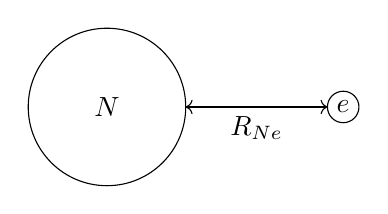
\begin{tikzpicture}
\draw (5,5) circle (1.0);
\node[] at (5,5) {$N$};
\node[] at (8,5) {$e$};
%\text (5,5) {$Z$};
\draw (8,5) circle(0.2);
\path[<->] (6,5) edge node[below] {$R_{Ne}$} (7.8,5);
\end{tikzpicture}
\end{figure}
\end{frame}


\begin{frame}
\frametitle{Le système}
L'interaction entre le proton (charge $Ze$ et l'électron (charge e) se décrit par 

\begin{equation}
V_{Ne}=-\frac{Ze^2}{4\pi\epsilon_0r}
\end{equation}
o\'u $e$ est la charge de l'électron, $Z$ est la charge du noyau, $epsilon_0$ est la permitivité du vide et $R_{Ne}$ est la distance qui sépare l'électron du noyau

\end{frame}
\section{L'hamiltonien}
\begin{frame}
On s'intéresse ici à l'électron en interaction avec le proton. Ce dernier est vu comme une charge immobile. On traitera en premier lieu la fonction radiale. L'hamiltonien est

\begin{equation}
\frametitle{Le système}
\hat{H}=\frac{1}{2m}\frac{\partial^2}{\partial x^2}-\frac{Ze^2}{4\pi\epsilon_0r}
\end{equation}



\end{frame}


\end{document}



